\documentclass[border=2mm]{standalone}
\usepackage{tikz}
\usepackage{tkz-euclide}
\usetikzlibrary{quotes,angles}

\begin{document}
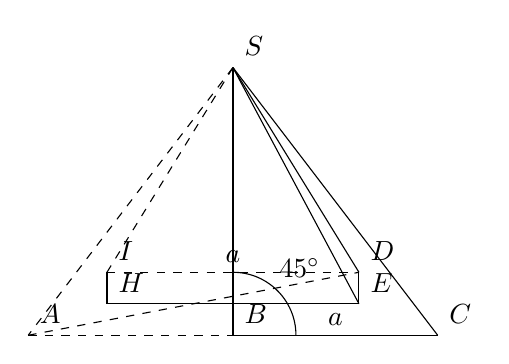
\begin{tikzpicture}
\coordinate (S) at (3.40, -0.40);
\coordinate (A) at (0.80, -3.80);
\coordinate (B) at (3.40, -3.80);
\coordinate (C) at (6.00, -3.80);
\coordinate (D) at (5.00, -3.00);
\coordinate (I) at (1.80, -3.00);
\coordinate (H) at (1.80, -3.40);
\coordinate (E) at (5.00, -3.40);
\draw[solid] (S) -- (B);
\draw[solid] (S) -- (C);
\draw[solid] (S) -- (D);
\draw[solid] (S) -- (E);
\draw[solid] (B) to["$a$"] (C);
\draw[solid] (I) -- (H);
\draw[solid] (H) -- (E);
\draw[solid] (E) -- (D);
\draw[dashed] (S) -- (A);
\draw[dashed] (S) -- (I);
\draw[dashed] (A) -- (B);
\draw[dashed] (A) -- (D);
\draw[dashed] (I) to["$a$"] (D);
\tkzMarkAngle[size=0.8, mark=none](C,B,S)
\tkzLabelAngle[pos=1.2](C,B,S){$45^\circ$}
\node[above right=1pt of S] {$S$};
\node[above right=1pt of A] {$A$};
\node[above right=1pt of B] {$B$};
\node[above right=1pt of C] {$C$};
\node[above right=1pt of D] {$D$};
\node[above right=1pt of I] {$I$};
\node[above right=1pt of H] {$H$};
\node[above right=1pt of E] {$E$};
\end{tikzpicture}
\end{document}